\chapter{Traceplots}
\label{sec:first-app}
\section{Normal model}

\begin{figure}[H]%
    \centering
    \subfloat[A]{\includegraphics[scale=0.3, page = 3]{figures/Normal/naive_compared1.pdf}}%
    \qquad
    \subfloat[B]{\includegraphics[scale=0.3, page = 3]{figures/Normal/flyMC_compared1.pdf}}%
    \newline
    \subfloat[C]{\includegraphics[scale=0.3, page = 3]{figures/Normal/confidence_compared1.pdf}}%
    \qquad
    \subfloat[D]{\includegraphics[scale=0.3, page = 3]{figures/Normal/confidence_w_pr_compared1.pdf}}%
    \caption{All plots A-D shows a Metropolis-Hastings chain, chain 1, plotted together with one other method. In A, chain 2 is the naive subsampler. In B, chain 2 is the Firefly, Figure C is the Bardenet et al. 2014 subsampler and D is the Bardenet et al. 2017 subsampler. $\theta
   ^{\left(0\right)}= \left(-0.2, -0.05\right)$}%
    \label{fig:compare_theta1_normal}%
\end{figure}





\begin{figure}%
   \centering
    \subfloat[$\theta_{init} = \theta_1$]{\includegraphics[scale=0.3, page = 3]{figures/Normal/10k_04_06_theta1.pdf}}%
    \qquad
    \subfloat[$\theta_{init} = \theta_2$]{\includegraphics[scale=0.3, page = 3]{figures/Normal/10k_12_06_theta2.pdf}}%
    \newline
    \subfloat[$\theta_{init} = \theta_3$]{\includegraphics[scale=0.3, page = 3]{figures/Normal/10k_12_06_theta3.pdf}}%
    \qquad
    \subfloat[$\theta_{init} = \theta_4$]{\includegraphics[scale=0.3, page = 3]{figures/Normal/10k_12_06_theta4.pdf}}%
    \newline
     \subfloat[$\theta_{init} = \theta_5$]{\includegraphics[scale=0.3, page = 3]{figures/Normal/10k_12_06_theta5.pdf}}%
    \caption{Chains for all methods, with different starting values for $\theta$.  }%
    \label{fig:chain_10k_04_06_normal}%
\end{figure}



\begin{figure}%
   \centering
    \subfloat[$\theta_{init} = \theta_1$]{\includegraphics[scale=0.3, page = 3]{figures/Normal/50k_04_06_theta1.pdf}}%
    \qquad
    \subfloat[$\theta_{init} = \theta_2$]{\includegraphics[scale=0.3, page = 3]{figures/Normal/50k_04_06_theta2.pdf}}%
    \newline
    \subfloat[$\theta_{init} = \theta_3$]{\includegraphics[scale=0.3, page = 3]{figures/Normal/50k_04_06_theta3.pdf}}%
    \qquad
    \subfloat[$\theta_{init} = \theta_4$]{\includegraphics[scale=0.3, page = 3]{figures/Normal/50k_04_06_theta4.pdf}}%
    \newline
     \subfloat[$\theta_{init} = \theta_5$]{\includegraphics[scale=0.3, page = 3]{figures/Normal/50k_04_06_theta5.pdf}}%
    \caption{Chains for all methods, with different starting values for $\theta$.  }%
    \label{fig:chain_50k_04_06_normal}%
\end{figure}



\section{Simple logistic regression}
\begin{figure}[H]%
    \centering
    \subfloat[A]{\includegraphics[scale=0.3, page = 3]{figures/ComparisonLogistic/naive_compared1.pdf}}%
    \qquad
    \subfloat[B]{\includegraphics[scale=0.3, page = 3]{figures/ComparisonLogistic/Firefly_compared1.pdf}}%
    \newline
    \subfloat[C]{\includegraphics[scale=0.3, page = 3]{figures/ComparisonLogistic/confidence_compared1.pdf}}%
    \qquad
    \subfloat[D]{\includegraphics[scale=0.3, page = 3]{figures/ComparisonLogistic/confidence_w_proxy_compared1.pdf}}%
    \caption{All plots A-D shows a Metropolis-Hastings chain, chain 1, plotted together with one other method. In Figure \ref{fig:compare_theta1}.A, chain 2 is the naive subsampler. In Figure\ref{fig:compare_theta1}.B, chain 2 is the Firefly, Figure \ref{fig:compare_theta1}.C is the Bardenet et al. 2014 subsampler and Figure \ref{fig:compare_theta1}.D is the Bardenet et al. 2017 subsampler. $\theta
   ^{\left(0\right)} = \left(-1,-2\right)$}%
    \label{fig:compare_theta1}%
\end{figure}

\begin{figure}[H]%
    \centering
    \subfloat[A]{\includegraphics[scale=0.3, page = 3]{figures/ComparisonLogistic/naive_compared2.pdf}}%
    \qquad
    \subfloat[B]{\includegraphics[scale=0.3, page = 3]{figures/ComparisonLogistic/Firefly_compared2.pdf}}%
    \newline
    \subfloat[C]{\includegraphics[scale=0.3, page = 3]{figures/ComparisonLogistic/confidence_compared2.pdf}}%
    \qquad
    \subfloat[D]{\includegraphics[scale=0.3, page = 3]{figures/ComparisonLogistic/confidence_w_proxy_compared2.pdf}}%
    \caption{All plots A-D shows a Metropolis-Hastings chain, chain 1, plotted together with one other method. In Figure \ref{fig:compare_theta2}.A, chain 2 is the naive subsampler. In Figure\ref{fig:compare_theta2}.B, chain 2 is the Firefly, Figure \ref{fig:compare_theta2}.C is the Bardenet et al. 2014 subsampler and Figure \ref{fig:compare_theta2}.D is the Bardenet et al. 2017 subsampler. $\theta
   ^{\left(0\right)} = \left(0.9,1.8\right)$}%
    \label{fig:compare_theta2}%
\end{figure}



\begin{figure}%
    \centering
    \subfloat[$\theta_{init} = \theta_1$]{\includegraphics[scale=0.3, page = 3]{figures/10k_iterations_02_06_theta1.pdf}}%
    \qquad
    \subfloat[$\theta_{init} = \theta_2$]{\includegraphics[scale=0.3, page = 3]{figures/10k_iterations_02_06_theta2.pdf}}%
    \newline
    \subfloat[$\theta_{init} = \theta_3$]{\includegraphics[scale=0.3, page = 3]{figures/10k_iterations_02_06_theta3.pdf}}%
    \qquad
    \subfloat[$\theta_{init} = \theta_4$]{\includegraphics[scale=0.3, page = 3]{figures/10k_iterations_02_06_theta4.pdf}}%
    \caption{Simulated values of $\beta_1$ and $\beta_2$ through the 10000 iterations, with a $20\%$ burn-in}%
    \label{fig:chain_10k_02_06}%
\end{figure}



\begin{figure}%
    \centering
    \subfloat[$\theta_{init} = \theta_1$]{\includegraphics[scale=0.3, page = 3]{figures/50k_iterations_02_06_theta1.pdf}}%
    \qquad
    \subfloat[$\theta_{init} = \theta_2$]{\includegraphics[scale=0.3, page = 3]{figures/50k_iterations_02_06_theta2.pdf}}%
    \newline
    \subfloat[$\theta_{init} = \theta_3$]{\includegraphics[scale=0.3, page = 3]{figures/50k_iterations_02_06_theta3.pdf}}%
    \qquad
    \subfloat[$\theta_{init} = \theta_4$]{\includegraphics[scale=0.3, page = 3]{figures/50k_iterations_02_06_theta4.pdf}}%
    \caption{Simulated values of $\beta_1$ and $\beta_2$ through the 10000 iterations, with a $20\%$ burn-in}%
    \label{fig:chain_50k_02_06}%
\end{figure}


\section{Multiple logistic regression}

\begin{figure}%
    \centering
    \subfloat{
    \includegraphics[scale=0.4, page = 5]{figures/multiple_logistic_regression/50k_iterations/02_06_theta1.pdf}}%
    \qquad
    \subfloat{
    \includegraphics[scale=0.4, page = 6]{figures/multiple_logistic_regression/50k_iterations/02_06_theta1.pdf}}%
    \caption{Simulated values of the $\beta$'s through the iterations with a $20\%$ burn-in $\theta^{\left(0\right)} = \mathbf{0}$}%
    \label{fig:chain_50k_02_06_theta1}%
\end{figure}



\begin{figure}%
    \centering
    \subfloat{
    \includegraphics[scale=0.4, page = 5]{figures/multiple_logistic_regression/50k_iterations/02_06_theta2.pdf}}%
    \qquad
    \subfloat{
    \includegraphics[scale=0.4, page = 6]{figures/multiple_logistic_regression/50k_iterations/02_06_theta2.pdf}}%
    \caption{Simulated values of the $\beta$'s through the iterations with a $20\%$ burn-in $\theta^{\left(0\right)} = \mathbf{1}$}%
    \label{fig:chain_50k_02_06_theta2}%
\end{figure}


\begin{figure}%
    \centering
    \subfloat{
    \includegraphics[scale=0.4, page = 5]{figures/multiple_logistic_regression/50k_iterations/02_06_theta3.pdf}}%
    \qquad
    \subfloat{
    \includegraphics[scale=0.4, page = 6]{figures/multiple_logistic_regression/50k_iterations/02_06_theta3.pdf}}%
    \caption{Simulated values of the $\beta$'s through the iterations with a $20\%$ burn-in $\theta^{\left(0\right)} = \theta$}%
    \label{fig:chain_50k_02_06_theta3}%
\end{figure}


